\title{triangulation with epipolar curves}



\newcommand{\1}{\mathbf{1}}
\newcommand{\R}{\mathbf{R}}
\newcommand{\T}{\mathbf{T}}
\newcommand{\Z}{\mathbf{Z}}
\newcommand{\ud}{\mathrm{d}}
\newcommand{\ds}{\displaystyle}
\def\argmin{\mathop{\rm argmin}}

% 0. Overview
% 1. Epipolar projection algorithm
% 2. Interpretation in terms of approximate Newton method
% 3. Linearized versions (including formulas)
% 4. Experiments with tokyo tower
% 5. Relationship with bundle adjustment

\section{Overiew}

An orbiting camera acquires two images of the same point in the surface of a
planet.  The camera platform is well-calibrated, thus the position and the
orientation at each acquisition are known.  By solving a
simple~\emph{triangulation} problem, we can recover the 3D position of that
point in the surface of the planet.
There are two sources of error: the calibration of the acquisition, and the
localization of the point within the domain of both images.  In this note we
study how each of these errors affects various triangulation methods.
The similar---and more interesting---problem of triangulating at once a large
set of points (bundle adjustment) is not treated here.

This is the acquisition setting:
\begin{center}
	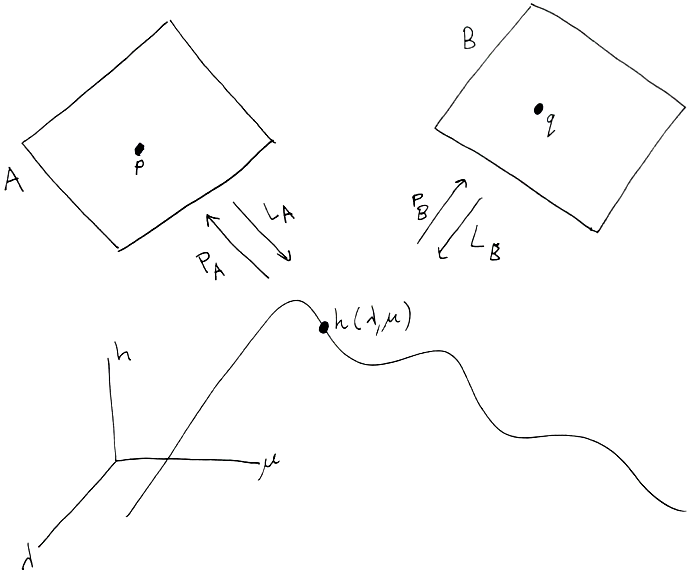
\includegraphics[width=0.6\linewidth]{tworpcs.png}
\end{center}
In words: each image $(A,B)$ is decorated with its
projection~$P:(\lambda,\mu,h)\mapsto(i,j)$ and
localization~$L:(i,j,h)\mapsto(\lambda,\mu,h)$ functions.  The triangulation
problem consists in finding the 3D coordinates~$(\lambda,\mu,h)$ of a point
given the observations~$p$,~$q$ of that point on each image.


\clearpage

{\bf Equivalent criteria:}\\
\begin{tabular}{l|l}
condition & dimensions \\
\hline
$L_A(p,h)=L_B(q,h)$  & 2 equations, 1 unknown\\
$P_B(L_A(p,h),h)=q$  & 2 equations, 1 unknown\\
$P_A(L_B(q,h),h)=p$  & 2 equations, 1 unknown\\
$L_A(p,h)=(x_1,x_2)=L_B(p,h)$ & 4 equations, 3 unknowns\\
$p=P_A(x),\ q=P_B(x)$ & 4 equations, 3 unknowns\\
\end{tabular}

{\bf Numeric criteria (not equivalent!):}\\
\begin{tabular}{l|l|l}
	criterion & name & output\\
	\hline
	$\ds\argmin_h\ds\left\|P_B(L_A(p,h),h)-q\right\|_B^2$ &
	epipolar error on B & $L_A(p,h)$\\
	$\ds\argmin_h\left\|P_A(L_B(q,h),h)-p\right\|_A^2$ &
	epipolar error on A &$L_B(q,h)$\\
	$\ds\argmin_h
	\left\|P_B(L_A(p,h),h)-q\right\|_B^2
	+
	\left\|P_A(L_B(q,h),h)-p\right\|_A^2 $ &
	symmetric epipolar error & $(?\,,\ ?\,,\ h)$ \\
	$\ds\argmin_h\left(\min_{h'}\left\|L_A(p,h)-L_B(q,h')\right\|^2_{\R^3}\right)$ &
	geometric error from $p$ & $L_A(p,h)$ \\
	$\ds\argmin_h\left(\min_{h'}\left\|L_A(p,h')-L_B(q,h)\right\|^2_{\R^3}\right)$ &
	geometric error from $q$ & $L_B(q,h)$ \\
	$\ds\argmin_h\left\|L_A(p,h)-L_B(p,h)\right\|_{\R^3}^2$ &
	horizontal geometric error & $(?\,,\ ?\,,\ h)$ \\
	$\ds\argmin_x\left(
		\left\|P_A(x)-p\right\|^2_A
		+
		\left\|P_B(x)-q\right\|^2_B
	\right)$ &
	minimal reprojection error & $x$\\
	%\tiny
	$\ds\argmin_x\left(
	\min_{h'}\left\|L_A(p,h')-x\right\|^2_{\R^3}
	+
	\min_{h'}\left\|L_B(q,h')-x\right\|^2_{\R^3}
	\right)$ & minimal geometric error & $x$
\end{tabular}



% vim:set tw=77 filetype=tex spell spelllang=en sw=2 ts=2:
